\documentclass[12pt,halfline,a4paper,]{ouparticle}

% Packages I think are necessary for basic Rmarkdown functionality
\usepackage{hyperref}
\usepackage{graphicx}
\usepackage{listings}
\usepackage{color}
\usepackage{fancyvrb}
\usepackage{framed}

%% To allow better options for figure placement
%\usepackage{float}

% Packages that are supposedly required by OUP sty file
\usepackage{amssymb, amsmath, geometry, amsfonts, verbatim, endnotes, setspace}

% For code highlighting I think
\DefineVerbatimEnvironment{Highlighting}{Verbatim}{commandchars=\\\{\}}
\definecolor{shadecolor}{RGB}{248,248,248}
\newenvironment{Shaded}{\begin{snugshade}}{\end{snugshade}}
\newcommand{\AlertTok}[1]{\textcolor[rgb]{0.94,0.16,0.16}{#1}}
\newcommand{\AnnotationTok}[1]{\textcolor[rgb]{0.56,0.35,0.01}{\textbf{\textit{#1}}}}
\newcommand{\AttributeTok}[1]{\textcolor[rgb]{0.77,0.63,0.00}{#1}}
\newcommand{\BaseNTok}[1]{\textcolor[rgb]{0.00,0.00,0.81}{#1}}
\newcommand{\BuiltInTok}[1]{#1}
\newcommand{\CharTok}[1]{\textcolor[rgb]{0.31,0.60,0.02}{#1}}
\newcommand{\CommentTok}[1]{\textcolor[rgb]{0.56,0.35,0.01}{\textit{#1}}}
\newcommand{\CommentVarTok}[1]{\textcolor[rgb]{0.56,0.35,0.01}{\textbf{\textit{#1}}}}
\newcommand{\ConstantTok}[1]{\textcolor[rgb]{0.00,0.00,0.00}{#1}}
\newcommand{\ControlFlowTok}[1]{\textcolor[rgb]{0.13,0.29,0.53}{\textbf{#1}}}
\newcommand{\DataTypeTok}[1]{\textcolor[rgb]{0.13,0.29,0.53}{#1}}
\newcommand{\DecValTok}[1]{\textcolor[rgb]{0.00,0.00,0.81}{#1}}
\newcommand{\DocumentationTok}[1]{\textcolor[rgb]{0.56,0.35,0.01}{\textbf{\textit{#1}}}}
\newcommand{\ErrorTok}[1]{\textcolor[rgb]{0.64,0.00,0.00}{\textbf{#1}}}
\newcommand{\ExtensionTok}[1]{#1}
\newcommand{\FloatTok}[1]{\textcolor[rgb]{0.00,0.00,0.81}{#1}}
\newcommand{\FunctionTok}[1]{\textcolor[rgb]{0.00,0.00,0.00}{#1}}
\newcommand{\ImportTok}[1]{#1}
\newcommand{\InformationTok}[1]{\textcolor[rgb]{0.56,0.35,0.01}{\textbf{\textit{#1}}}}
\newcommand{\KeywordTok}[1]{\textcolor[rgb]{0.13,0.29,0.53}{\textbf{#1}}}
\newcommand{\NormalTok}[1]{#1}
\newcommand{\OperatorTok}[1]{\textcolor[rgb]{0.81,0.36,0.00}{\textbf{#1}}}
\newcommand{\OtherTok}[1]{\textcolor[rgb]{0.56,0.35,0.01}{#1}}
\newcommand{\PreprocessorTok}[1]{\textcolor[rgb]{0.56,0.35,0.01}{\textit{#1}}}
\newcommand{\RegionMarkerTok}[1]{#1}
\newcommand{\SpecialCharTok}[1]{\textcolor[rgb]{0.00,0.00,0.00}{#1}}
\newcommand{\SpecialStringTok}[1]{\textcolor[rgb]{0.31,0.60,0.02}{#1}}
\newcommand{\StringTok}[1]{\textcolor[rgb]{0.31,0.60,0.02}{#1}}
\newcommand{\VariableTok}[1]{\textcolor[rgb]{0.00,0.00,0.00}{#1}}
\newcommand{\VerbatimStringTok}[1]{\textcolor[rgb]{0.31,0.60,0.02}{#1}}
\newcommand{\WarningTok}[1]{\textcolor[rgb]{0.56,0.35,0.01}{\textbf{\textit{#1}}}}

% For making Rmarkdown lists
\providecommand{\tightlist}{%
  \setlength{\itemsep}{0pt}\setlength{\parskip}{0pt}}


% Part for setting citation format package: natbib
\usepackage{natbib}
\bibliographystyle{plainnat}

% Part for setting citation format package: biblatex

% Pandoc header

\begin{document}

\title{Do reaction times differ between women and men?}

\author{%
\name{Owen L. Petchey}\address{University of Zurich}\email{\href{mailto:owen.petchey@ieu.uzh.ch}{owen.petchey@ieu.uzh.ch}}\thanks{Corresponding author; Email: \href{mailto:owen.petchey@ieu.uzh.ch}{owen.petchey@ieu.uzh.ch}}
\and
\name{Your Name}\address{Your University}\email{\href{mailto:your@name.com}{your@name.com}}
}

\abstract{This is the abstract.

It consists of two paragraphs.}

\date{\today}

\keywords{key; dictionary; word}

\maketitle



\hypertarget{introduction}{%
\section{Introduction}\label{introduction}}

\hypertarget{materials-and-methods}{%
\section{Materials and methods}\label{materials-and-methods}}

\hypertarget{results}{%
\section{Results}\label{results}}

Numbers of sampled women and men, and the mean and median reaction time,
and the standard error of the mean (SEM) (Table
\ref{tab:summary-stats}.)

\begin{table}[ht]
\centering
\begin{tabular}{rlrrrr}
  \hline
 & Gender & number & mean & median & SEM \\ 
  \hline
1 & Female & 127 & 322.92 & 317.00 & 5.93 \\ 
  2 & Male &  66 & 302.90 & 296.00 & 5.71 \\ 
   \hline
\end{tabular}
\caption{This is the table caption} 
\label{tab:summary-stats}
\end{table}

You can reference this figure as follows: Fig. \ref{fig:prt-histograms}.

\begin{figure}[p]

{\centering 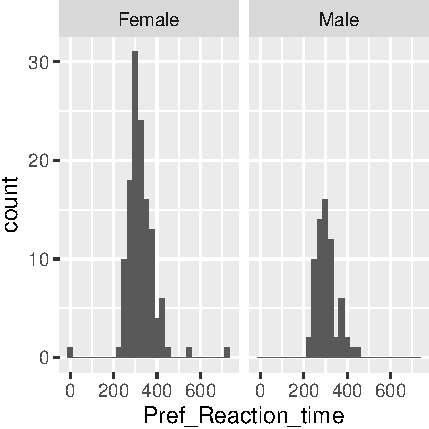
\includegraphics[width=0.5\linewidth]{manuscript_reaction_times_2020_files/figure-latex/prt-histograms-1} 

}

\caption{This is the first figure.}\label{fig:prt-histograms}
\end{figure}

We filtered the reaction time data to remove those less than 50 and
greater than 500 milliseconds.

You can reference this figure as follows: Fig. \ref{fig:prt-boxplot}.

\begin{figure}[p]

{\centering 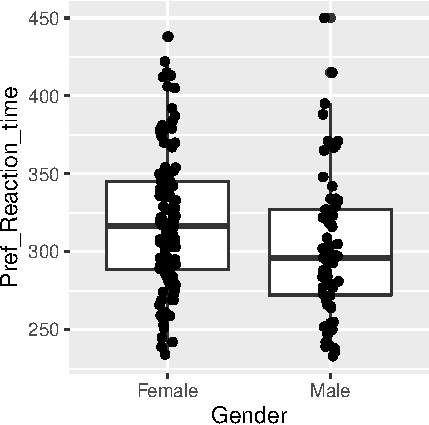
\includegraphics[width=0.5\linewidth]{manuscript_reaction_times_2020_files/figure-latex/prt-boxplot-1} 

}

\caption{This is the second figure, using filtered data.}\label{fig:prt-boxplot}
\end{figure}

T-test on the filtered data: t = 3.

\hypertarget{discussion}{%
\section{Discussion}\label{discussion}}

\hypertarget{references}{%
\section{References}\label{references}}

\hypertarget{below-here-is-information-about-how-to-write-in-markdown-put-in-figures-cross-reference-etc.}{%
\section{****Below here is information about how to write in markdown,
put in figures, cross reference,
etc.}\label{below-here-is-information-about-how-to-write-in-markdown-put-in-figures-cross-reference-etc.}}

\hypertarget{introduction-1}{%
\section{Introduction}\label{introduction-1}}

This template is based on the generic OUP template available
\href{https://academic.oup.com/icesjms/pages/General_Instructions}{here}.
The original OUP sample tex document, providing more details on prefered
formatting for LaTeX documents, is included with the template in the
file \texttt{ouparticle\_sample.tex}.

Here are two sample references: \citeauthor{Feynman1963118}
\citetext{\citeyear{Feynman1963118}; \citealp{Dirac1953888}}.
Bibliography will appear at the end of the document.

\hypertarget{materials-and-methods-1}{%
\section{Materials and methods}\label{materials-and-methods-1}}

An equation with a label for cross-referencing:

\begin{equation}\label{eq:eq1}
\int^{r_2}_0 F(r,\varphi){\rm d}r\,{\rm d}\varphi = [\sigma r_2/(2\mu_0)]
\int^{\infty}_0\exp(-\lambda|z_j-z_i|)\lambda^{-1}J_1 (\lambda r_2)J_0
(\lambda r_i\,\lambda {\rm d}\lambda)
\end{equation}

This equation can be referenced as follows: Eq. \ref{eq:eq1}

\hypertarget{a-subsection}{%
\subsection{A subsection}\label{a-subsection}}

A numbered list:

\begin{enumerate}
\def\labelenumi{\arabic{enumi})}
\tightlist
\item
  First point
\item
  Second point

  \begin{itemize}
  \tightlist
  \item
    Subpoint
  \end{itemize}
\end{enumerate}

A bullet list:

\begin{itemize}
\tightlist
\item
  First point
\item
  Second point
\end{itemize}

\hypertarget{results-1}{%
\section{Results}\label{results-1}}

Generate a figure.

\begin{Shaded}
\begin{Highlighting}[]
\KeywordTok{plot}\NormalTok{(}\DecValTok{1}\OperatorTok{:}\DecValTok{10}\NormalTok{,}\DataTypeTok{main=}\StringTok{"Some data"}\NormalTok{,}\DataTypeTok{xlab=}\StringTok{"Distance (cm)"}\NormalTok{,}\DataTypeTok{ylab=}\StringTok{"Time (hours)"}\NormalTok{)}
\end{Highlighting}
\end{Shaded}

\begin{figure}[p]
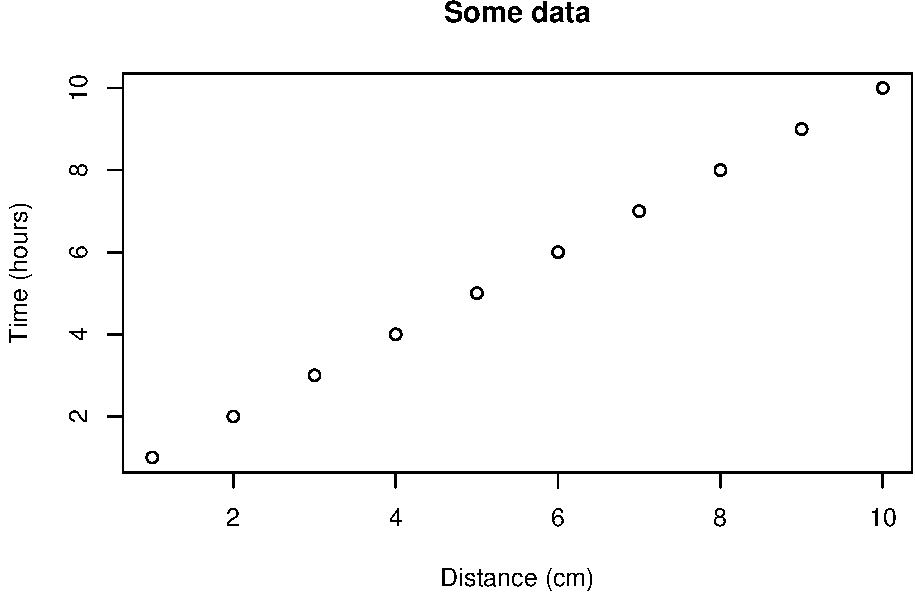
\includegraphics[width=1\linewidth]{manuscript_reaction_times_2020_files/figure-latex/fig1-1} \caption{This is the first figure.}\label{fig:fig1}
\end{figure}

You can reference this figure as follows: Fig. \ref{fig:fig1}.

\begin{Shaded}
\begin{Highlighting}[]
\KeywordTok{plot}\NormalTok{(}\DecValTok{1}\OperatorTok{:}\DecValTok{5}\NormalTok{,}\DataTypeTok{pch=}\DecValTok{19}\NormalTok{,}\DataTypeTok{main=}\StringTok{"Some data"}\NormalTok{,}\DataTypeTok{xlab=}\StringTok{"Distance (cm)"}\NormalTok{,}\DataTypeTok{ylab=}\StringTok{"Time (hours)"}\NormalTok{)}
\end{Highlighting}
\end{Shaded}

\begin{figure}[p]
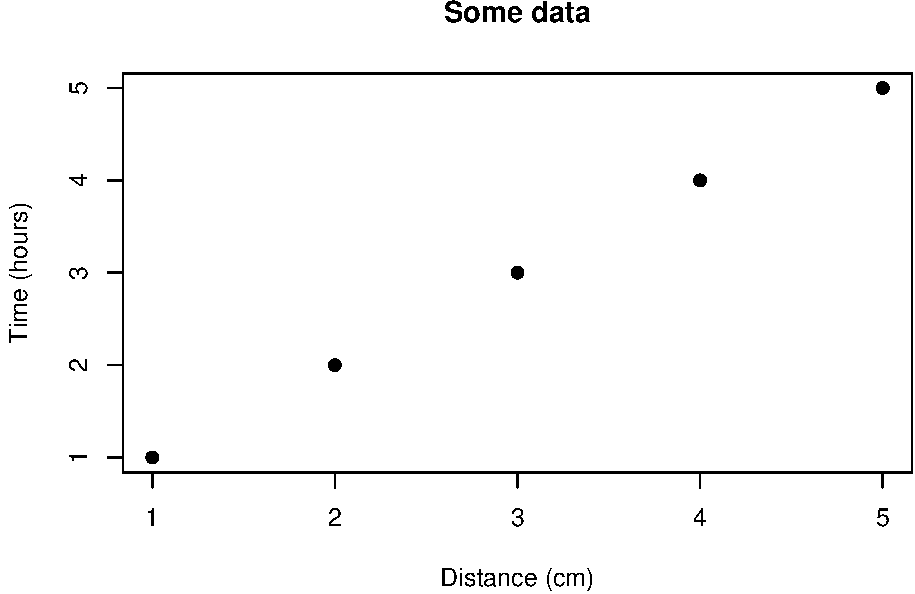
\includegraphics[width=1\linewidth]{manuscript_reaction_times_2020_files/figure-latex/fig2-1} \caption{This is the second figure.}\label{fig:fig2}
\end{figure}

Reference to second figure: Fig. \ref{fig:fig2}

Generate a table.

\begin{Shaded}
\begin{Highlighting}[]
\NormalTok{df =}\StringTok{ }\KeywordTok{data.frame}\NormalTok{(}\DataTypeTok{ID=}\DecValTok{1}\OperatorTok{:}\DecValTok{3}\NormalTok{,}\DataTypeTok{code=}\NormalTok{letters[}\DecValTok{1}\OperatorTok{:}\DecValTok{3}\NormalTok{])}
\KeywordTok{print}\NormalTok{(}\KeywordTok{xtable}\NormalTok{(df,}\DataTypeTok{caption=}\StringTok{"This is the table caption"}\NormalTok{,}\DataTypeTok{label=}\StringTok{"tab:tab1"}\NormalTok{),}
      \DataTypeTok{comment=}\OtherTok{FALSE}\NormalTok{)}
\end{Highlighting}
\end{Shaded}

\begin{table}[ht]
\centering
\begin{tabular}{rrl}
  \hline
 & ID & code \\ 
  \hline
1 &   1 & a \\ 
  2 &   2 & b \\ 
  3 &   3 & c \\ 
   \hline
\end{tabular}
\caption{This is the table caption} 
\label{tab:tab1}
\end{table}

You can reference this table as follows: Table \ref{tab:tab1}.

\hypertarget{discussion-1}{%
\section{Discussion}\label{discussion-1}}

You can cross-reference sections and subsections as follows: Section
\ref{materials-and-methods} and Section \ref{a-subsection}.

\textbf{\emph{Note:}} the last section in the document will be used as
the section title for the bibliography.


\begin{notes}[Acknowledgements]
This is an acknowledgement.

It consists of two paragraphs.
\end{notes}


\renewcommand\refname{References}

\bibliography{mybibfile.bib}



\end{document}
